\documentclass[preprint,authoryear,12pt]{noelsarticle}
%\documentclass[preprint,12pt]{elsarticle}
%\documentclass[final,3p,times,authoryear]{elsarticle}
%\documentclass[final,3p,times]{elsarticle}

\usepackage{tikz}
\usepackage{hyperref}
\usepackage{verbatim}
\usepackage{comment}
\usepackage{boxedminipage}
\usepackage{amssymb}
\usepackage{listings,lsthaskell,lstprolog,lstegl,lstesl,lstfsml}

\newcommand{\m}[1]{\ensuremath{\mathit{#1}}}
\newcommand{\concept}[1]{\emph{#1}}
\definecolor{codebackground}{rgb}{0.97,0.97,0.97}
\definecolor{gray}{rgb}{0.5,0.5,0.5}
\definecolor{keyword}{rgb}{0.5,0.0,0.5}
\definecolor{comment}{rgb}{0.3,0.5,0.3}
\definecolor{code}{rgb}{0.0,0.0,0.3}
\definecolor{ncode}{rgb}{0.0,0.3,0.3}
\definecolor{scode}{rgb}{0.3,0.0,0.3}
\definecolor{static}{rgb}{0.0,0.0,0.3}
\newcommand{\ncode}[1]{\texttt{\textup{\color{ncode}#1}}}
\newcommand{\jcode}[1]{\texttt{\textup{\color{code}#1}}}
\newcommand{\scode}[1]{\texttt{\textup{\color{scode}#1}}}
\newcommand{\static}[1]{\texttt{\textsl{\color{static}#1}}}

\newcommand{\codefigure}[3]{
\begin{figure}[t!]
\begin{boxedminipage}{\hsize}
\mbox{}\hfill{}{\small\textsf{\href{http://github.com/slebok/slepro/tree/master/#2}{#2}}}
\lstinputlisting[language=#3]{../../#2}
\end{boxedminipage}
\caption{#1.}
\label{#2}
\end{figure}}

\lstset{%
  fontadjust=true,%
  showstringspaces=false,%
  keywordstyle=\color{keyword},%
  commentstyle=\color{comment}\rmfamily\itshape\small,%
  columns=fullflexible,%
  tabsize=2,
%  numbers=left,                   % where to put the line-numbers
  numberstyle=\tiny\color{gray},  % the style that is used for the line-numbers
  backgroundcolor=\color{codebackground},
  stepnumber=2,                   % the step between two line-numbers
%  numbersep=5pt,                  % how far the line-numbers are from the code
 % aboveskip=1.5\medskipamount,%
 % belowskip=1.5\medskipamount,
aboveskip = 0pt,
belowskip = 0pt,
  %breaklines=true
}

\lstdefinestyle{haskell}{
  language=Haskell,
  basicstyle=\small\color{ncode}\ttfamily,%
}

\lstdefinestyle{prolog}{
  language=Prolog,
  basicstyle=\small\color{ncode}\ttfamily,%
}

\newcommand{\wikipediafn}[2]{\footnote{\url{#1}---last visited #2.}}
\newcommand{\ooo}[1]{\textsf{101#1}}

%% \biboptions{comma,round}
% \biboptions{}

\begin{document}

\begin{frontmatter}

\title{Another DSL primer}

\author{Ralf L\"ammel}

\address{Software Languages Team\\University of Koblenz-Landau, Germany}

\begin{abstract}
  We model a domain-specific language FSML for Finite State Machines
  (FSMs). The language model encompasses concrete a textual syntax, a
  term-based abstract syntax, a graph-based visual syntax, extra
  constraints for well-formedness, a simulation semantics, and a
  code-generation semantics for representing and executing FSMs in
  Java. The key motivation for the present model of FSML to be
  explainable exhaustively in terms of simple formalisms and idioms,
  all layered on top of Prolog.

\bigskip

\noindent
\textbf{Acknowledgement}: {\small This document and the underlying
  development are parts of a broader effort on language modeling and
  software language engineering---joint work with \emph{Anya Helene
    Bagge}, University of Bergen. Helpful interaction with and
  feedback by Andrei Varanovich, University of Koblenz-Landau, is also
  gratefully acknowledged.}

\medskip

\noindent
\textbf{Version}

0.000001 as of 4 November 2013.

\medskip

\noindent
\textbf{Repository location of document}: 

\url{https://github.com/slebok/slepro/tree/master/docs/fsml}.
\end{abstract}

% \begin{keyword} 
% ???
% \end{keyword}

\end{frontmatter}

\pagebreak

%%%%%%%%%%%%%%%%%%%%%%%%%%%%%%%%%%%%%%%%%%%%%%%%%%

\tableofcontents

\pagebreak

%%%%%%%%%%%%%%%%%%%%%%%%%%%%%%%%%%%%%%%%%%%%%%%%%%

\section{Introducing FSML}

%%%%%%%%%%%%%%%%%%%%%%%%%%%%%%%%%%%%%%%%%%%%%%%%%%

\begin{figure}[t!]
\vspace{-77\in}
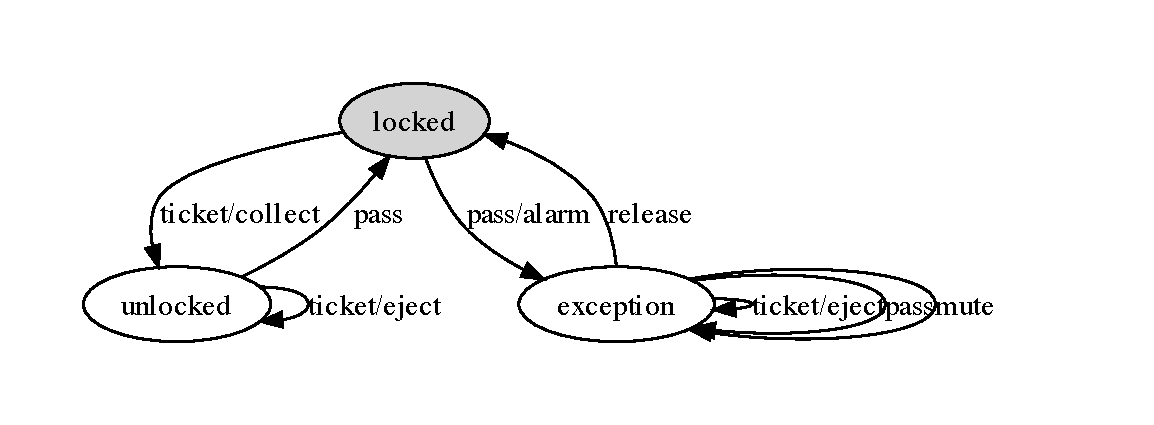
\includegraphics[width=\textwidth]{../../languages/fsml/sample-turnstile.pdf}
\vspace{-150\in}
\caption{A finite state machine for turnstiles.}
\label{F:turnstile}
\end{figure}

%%%%%%%%%%%%%%%%%%%%%%%%%%%%%%%%%%%%%%%%%%%%%%%%%%

Consider the visual representation of a finite state machine (FSM) for
a turnstile (as used in subway systems). The idea is, of course, that
the customer is supposed to insert a ticket before passing the
turnstile. Thus, the FSM assumes the initial state `locked'. (The
initial state is highlighted by using a filled ellipse.) The input
`ticket' (meaning the insertion of a ticket) causes a transition to
the state `unlocked' and the action `collect'. In this new state, the
input `pass' (meaning the attempt to pass the turnstile) causes a
transition back to the state `locked'. If the input `pass' was made in
the state `locked', then this causes a transition to the state
`exception' and an action `alarm'. The state `exception' rejects the
input `ticket'. The input `pass' does, of course, keeps one in the
state `exception'. The `alarm' can be muted with the input `mute'. We
return to the normal `locked' state upon the input `release'.

We will model a language FSML (FSM language) for modeling
FSMs. Specifically, we will model several aspects of FSML:

\begin{itemize}
\item The visual syntax as used in the figure; see \S\ref{S:visual}.
\item A textual syntax as an alternative concrete syntax; see \S\ref{S:textual}.
\item An abstract syntax useful for representation in programs; see \S\ref{S:abstract}.
\item Extra well-formedness constraints on the abstract syntax; see \S\ref{S:ok}.
\item A reference semantics for the simulation of FSMs; see \S\ref{S:semantics}.
\item A code generator translating FSMs into OO programs; see \S\ref{S:generator}.
\end{itemize}

This primer is concluded by some `food for thought' in
\S\ref{S:concl}. That is, we state shortcomings or issues of
incompleteness of the language model approach at hand, thereby also
motivating reproductions of the model as well as variations on the
model, possibly leveraging diverse metaprogramming settings.

%%%%%%%%%%%%%%%%%%%%%%%%%%%%%%%%%%%%%%%%%%%%%%%%%%

\section{The concrete textual syntax of FSML}
\label{S:textual}

\codefigure{%
The FSM of \autoref{F:turnstile} in concrete textual syntax}{%
languages/fsml/sample-turnstile.fsml}{%
fsml}

A textual syntax may break down an FSM into `state declarations',
i.e., states with the associated transitions. Each transition
identifies the relevant input, the optional action, and the target
state. In fact, if the target state is omitted, then this is taken to
mean that the transition's target is the current state. See
\autoref{languages/fsml/sample-turnstile.fsml} for an illustration.

\codefigure{%
Context-free grammar for the concrete syntax of FSML}{%
languages/fsml/cs.egl}{%
egl}

Let us define the syntax in terms of a context-free grammar. We use an
EGL grammar, where EGL stands for extended grammar language and can be
regarded as a variation on the Extended Backus Naur Form. EGL is an
ad-hoc grammar notation that is provided by the same project that
hosts the present FSML model. In particular, EGL grammars can be
executed for the purpose of parsing, but we omit all such details
here. See \autoref{languages/fsml/cs.egl} for the grammar. It can be
assumed that the concrete textual syntax, as illustrated in
\autoref{languages/fsml/sample-turnstile.fsml}, can be parsed indeed
with the present grammar.

%%%%%%%%%%%%%%%%%%%%%%%%%%%%%%%%%%%%%%%%%%%%%%%%%%

\section{The abstract syntax of FSML}
\label{S:abstract}

Eventually, we want to manipulate FSMs in (Prolog) programs. To this
end, we need a suitable abstract syntax. As an aside, there exist
metaprogramming systems that can leverage the concrete syntax
directly, without any need for a separate abstract syntax, but we will
adopt the simpler approach here to indeed use an abstract syntax. In
fact, we assume that abstract syntax trees are (Prolog) terms as in
the sense of term algebras or algebraic specifications.

\codefigure{%
The FSM of \autoref{F:turnstile} in abstract syntax}{%
languages/fsml/sample-turnstile-fsml.term}{%
prolog}

See \autoref{languages/fsml/sample-turnstile-fsml.term} for an
illustration. The abstract syntax describes a FSM as a list of state
declarations, which are in turn tuples (triplets) of the form (\m{V},
\m{Id}, \m{Ts}) where \m{V} is a Boolean saying whether the state is
initial, \m{Id} is the assigned id (name) of the state, and \m{Ts} is
a list of transitions. Each transition is a triplet of the form
(\m{In}, \m{A}, \m{To}) where \m{In} is the input for the transition,
\m{A} is the optional action and \m{To} is the target state. The
optionality of the action is represented such that the missing action
is represented by `[]' and the present action, e.g., `eject', is
represented by `[eject]'.

\codefigure{%
Signature for the abstract syntax of FSML}{%
languages/fsml/as.esl}{%
esl}

Let us define the abstract syntax in terms of a signature that defines
all valid FSM terms. We use an ESL signature, where ESL stands for
extended signature language and can be regarded as (quite) a variation
on notations familiar from algebraic specification or (less) a
variation on type systems used in logic or functional programming. ESL
is an ad-hoc signature notation that is provided by the same project
that hosts the present FSML model. In particular, ESL grammars can be
executed for conformance checking to see whether a given term conforms
to a given signature, but we omit all such details here. See
\autoref{languages/fsml/as.esl} for the signature. The term in
\autoref{languages/fsml/sample-turnstile-fsml.term} conforms indeed
to the present signature.

\codefigure{%
Concrete to abstract syntax mapping for FSML}{%
languages/fsml/cs-to-as.pro}{%
prolog}

As we intend to parse FSMs via the concrete textual syntax and to
manipulate FSMs though via the abstract term-based syntax, we need a
mapping from the former to the latter. Of course, both syntaxes are
very close to each other in terms of the nonterminals or types defined
and in terms of the structural breakdown. However, some fine details
need to be declared explicitly via a mapping so that parse trees
according to the earlier grammar are precisely mapped to terms that
conform to the signature for the abstract syntax. The mapping is
defined by a Prolog predicate \emph{fsmlMapping}; see the Prolog
clauses in \autoref{languages/fsml/cs-to-as.pro}.

The syntax definition approach of the present project assumes such
mappings are indeed predicates with three arguments \m{N}, \m{T1},
\m{T2} as follows. \m{N} is the nonterminal (according to the grammar
for the concrete syntax) whose parse trees are to be mapped, i.e.,
rewritten. \m{T1} is the (imploded) parse tree that just
systematically follows the structure of the grammar. \m{T2} is the
term that should be used in place of \m{T1}. The starting point is an
identity mapping; the mapping predicate only overwrites those cases
where the identity mapping is not appropriate. In
\autoref{languages/fsml/cs-to-as.pro}, the first clause replaces the
list-of-chars representation of FSM names by proper atoms (`strings').
The second clause replaces `initial' by `true' (and `noninitial' by
`false'); it also fills in the target state, when it is missing,
thereby taking care of some syntactic sugar, i.e., the permitted
omission of the target state when it equals the source state of a
transition.

%%%%%%%%%%%%%%%%%%%%%%%%%%%%%%%%%%%%%%%%%%%%%%%%%%

\section{Constraints on the abstract syntax}
\label{S:ok}

The concrete and abstract syntaxes so far do not cover some of the
constraints that we would naturally apply to FSMs. For instance, we
did not rule out so far that FSMs have multiple initial states, which
is probably not useful. Context-free grammars and signatures are
notoriously limited in expressiveness to model such constraints,
whereas they are convenient for the basic definition of structure. We
need to add extra constraints on top of (say) the abstract syntax
definition. In some communities, it is common to actually consider
these constraints to form part of the abstract syntax whereas we
follow another common view that such constraints are considered
separately as in well-formedness or well-typedness judgements used in
type systems for programming languages.

\codefigure{%
Overview of constraints imposed on FSML's abstract syntax}{%
languages/fsml/ok.pro}{%
prolog}

See \autoref{languages/fsml/ok.pro} for the Prolog specification
listing the named constraints that we consider here. Each constraint
gives rise to a separate predicate considered below. Here is short
summary. Constraint \emph{fsmSingleInitial} is meant to ensure that
there is only a single state declaration for an initial
state. Constraint \emph{fsmDistinctIds} is meant to ensure that the
state ids of the state declarations are distinct. Constraint
\emph{fsmResolvable} is meant to ensure that all referenced target
states are declared. Constraint \emph{fsmDeterministic} is meant
to ensure that each given input uniquely defines the target state to
be transitioned to, if any. Constraint \emph{fsmReachable} is meant to
ensure that all declared states are reachable from the
initial state. In \autoref{languages/fsml/ok.pro}, all constraint
predicates are surround by an application of the meta-predicate
\emph{require/1}, which is simply there for better error
reporting. That is, if the argument of \emph{require/1} fails, then
this is reported immediately, as opposed to simply propagating failure
silently.

\codefigure{%
There is only a single state declaration for an initial state}{%
languages/fsml/ok/initial.pro}{%
prolog}

\codefigure{%
The state ids of the state declarations are distinct}{%
languages/fsml/ok/distinct.pro}{%
prolog}

\codefigure{%
All referenced target states are declared}{%
languages/fsml/ok/resolvable.pro}{%
prolog}

\codefigure{%
Each given input uniquely defines the target state to be transitioned to, if any}{%
languages/fsml/ok/deterministic.pro}{%
prolog}

\codefigure{%
All declared states are reachable from the initial state}{%
languages/fsml/ok/reachable.pro}{%
prolog}

\codefigure{%
Fixed point computation needed in \autoref{languages/fsml/ok/reachable.pro}}{%
languages/fsml/ok/closure.pro}{%
prolog}

All constraints are specified in
\autoref{languages/fsml/ok/initial.pro}--\autoref{languages/fsml/ok/closure.pro}. The
constraints are relatively simple to express using Prolog's
meta-predicate \emph{findall/3} which serves here for queries into the
terms of the abstract syntax. For instance, in
\autoref{languages/fsml/ok/initial.pro}, we find all state ids from
state declarations with `true' for the initial component. Once this
set is retrieved that the resulting list is of length 1; thus, there
is exactly one initial.

The constraint for reachability
(\autoref{languages/fsml/ok/reachable.pro}--\autoref{languages/fsml/ok/closure.pro})
is somewhat interesting, as we have to model a fixed point computation
to find all states by repeated consideration of transition as to
whether the set of known to be reachable states implies more reachable
states. The fixed point criterion is here that we do not find
additional states; see \autoref{languages/fsml/ok/closure.pro}.

%%%%%%%%%%%%%%%%%%%%%%%%%%%%%%%%%%%%%%%%%%%%%%%%%%

\section{The reference semantics for FSML}
\label{S:semantics}

TBD

%%%%%%%%%%%%%%%%%%%%%%%%%%%%%%%%%%%%%%%%%%%%%%%%%%

\section{The code generator for FSML}
\label{S:generator}

TBD

%%%%%%%%%%%%%%%%%%%%%%%%%%%%%%%%%%%%%%%%%%%%%%%%%%

\section{The visual syntax of FSML}
\label{S:visual}

TBD

%%%%%%%%%%%%%%%%%%%%%%%%%%%%%%%%%%%%%%%%%%%%%%%%%%

\section{Food for thought}
\label{S:concl}

TBD

%%%%%%%%%%%%%%%%%%%%%%%%%%%%%%%%%%%%%%%%%%%%%%%%%%

{\small

%\nocite{FreeDictionary}
%\setlength{\bibsep}{4pt}
%\bibliographystyle{elsarticle-harv}
%\bibliographystyle{elsarticle-num}
%\bibliography{paper}

}

\end{document}
